\documentclass[10pt, a5paper]{article}
\usepackage{pdfpages}
\usepackage{parallel}
\usepackage[T2A]{fontenc}
\usepackage{ucs}
\usepackage[utf8x]{inputenc}
\usepackage[polish,english,russian]{babel}
\usepackage{hyperref}
\usepackage{rotating}
\usepackage[inner=2cm,top=1.8cm,outer=2cm,bottom=2.3cm,nohead]{geometry}
\usepackage{listings}
\usepackage{graphicx}
\usepackage{wrapfig}
\usepackage{longtable}
\usepackage{indentfirst}
\usepackage{array}
\newcolumntype{P}[1]{>{\raggedright\arraybackslash}p{#1}}
\frenchspacing
\usepackage{fixltx2e} %text sub- and superscripts
\usepackage{icomma} % коскі ў матэматычным рэжыме
\PreloadUnicodePage{4}

\newcommand{\longpage}{\enlargethispage{\baselineskip}}
\newcommand{\shortpage}{\enlargethispage{-\baselineskip}}

\def\switchlang#1{\expandafter\csname switchlang#1\endcsname}
\def\switchlangbe{
\let\saverefname=\refname%
\def\refname{Літаратура}%
\def\figurename{Іл.}%
}
\def\switchlangen{
\let\saverefname=\refname%
\def\refname{References}%
\def\figurename{Fig.}%
}
\def\switchlangru{
\let\saverefname=\refname%
\let\savefigurename=\figurename%
\def\refname{Литература}%
\def\figurename{Рис.}%
}

\hyphenation{admi-ni-stra-tive}
\hyphenation{ex-pe-ri-ence}
\hyphenation{fle-xi-bi-li-ty}
\hyphenation{Py-thon}
\hyphenation{ma-the-ma-ti-cal}
\hyphenation{re-ported}
\hyphenation{imp-le-menta-tions}
\hyphenation{pro-vides}
\hyphenation{en-gi-neering}
\hyphenation{com-pa-ti-bi-li-ty}
\hyphenation{im-pos-sible}
\hyphenation{desk-top}
\hyphenation{elec-tro-nic}
\hyphenation{com-pa-ny}
\hyphenation{de-ve-lop-ment}
\hyphenation{de-ve-loping}
\hyphenation{de-ve-lop}
\hyphenation{da-ta-ba-se}
\hyphenation{plat-forms}
\hyphenation{or-ga-ni-za-tion}
\hyphenation{pro-gramming}
\hyphenation{in-stru-ments}
\hyphenation{Li-nux}
\hyphenation{sour-ce}
\hyphenation{en-vi-ron-ment}
\hyphenation{Te-le-pathy}
\hyphenation{Li-nux-ov-ka}
\hyphenation{Open-BSD}
\hyphenation{Free-BSD}
\hyphenation{men-ti-on-ed}
\hyphenation{app-li-ca-tion}

\def\progref!#1!{\texttt{#1}}
\renewcommand{\arraystretch}{2} %Іначай формулы ў матрыцы зліпаюцца з лініямі
\usepackage{array}

\def\interview #1 (#2), #3, #4, #5\par{

\section[#1, #3, #4]{#1 -- #3, #4}
\def\qname{LVEE}
\def\aname{#1}
\def\q ##1\par{{\noindent \bf \qname: ##1 }\par}
\def\a{{\noindent \bf \aname: } \def\qname{L}\def\aname{#2}}
}

\def\interview* #1 (#2), #3, #4, #5\par{

\section*{#1\\{\small\rm #3, #4. #5}}

\def\qname{LVEE}
\def\aname{#1}
\def\q ##1\par{{\noindent \bf \qname: ##1 }\par}
\def\a{{\noindent \bf \aname: } \def\qname{L}\def\aname{#2}}
}

\switchlang{ru}
\begin{document}
\title{Основы IPv6}
\author{Ivan Semernik, Minsk, Belarus \footnote{\url{ivan.semernik@gmail.com}, \url {https://lvee.org/ru/abstracts/250}}}
\maketitle
\begin{abstract}
2016 is a year when exponential growth of world IPv6 adoption was confirmed. Fifth part of Global IP traffic going over IPv6 now. Per country adoption level of IPv6 is very different (from 0\% to almost 50\% in Europe region). Belarus is only 0,03\%. There are many reasons for that and poor technical knowledge of IPv6 is one of them.
\end{abstract}
IPv6 ~--- новая версия протокола IP, призванная решить проблемы, с которыми столкнулась предыдущая версия (IPv4) при её использовании в Интернете, за счёт использования 128 битной адресации вместо 32 битной. Протокол был разработан IETF. ~\cite{Semernik-0}

В настоящее время протокол IPv6 уже используется в нескольких десятках тысячах сетей по всему миру (более 40000 сетей на лето 2017 года), но пока ещё не получил столь широкого распространения в Интернете, как IPv4. 2016 год стал годом подтвержденного экспонетциального роста IPv6 подключений по всему миру. ~\cite{Semernik-1} На середину 2017 года доля IPv6 в общемировом сетевом трафике составляет около 18\%. ~\cite{Semernik-2}

Изображение: Прогноз исчерпания адресного пространства IPv4 региональными регистратурами, Geoff Huston / ipv4.potaroo.net



После того, как адресное пространство в IPv4 закончится, два стека протоколов — IPv6 и IPv4 — будут использоваться параллельно (IP dual stack), с постепенным увеличением доли трафика IPv6, по сравнению с IPv4.

При разработке нового протокола IPv6 были учтены многие проблемы и узкие места протокола IPv4.

Краткое сравнение IPv4  и IPv6 приведено в таблице.

\begin{table}
  \centering
  \begin{tabular}{ p{3cm} p{3cm} p{4cm} }
      							& IPv4 (c 1981) 	& IPv6 (c 1998) \\
     Разрядность  				&  32 бита 			& 128 бит  \\
     Пример адреса  			&  212.98.163.254  	&  2001:db8:6:56::53  \\
%     Год публикации 			&  1981  			&  1998  \\
     Адресное пространство:  	&  4 294 967 296 адресов  &  340 282 366 920 938 463 463 374 607 431 768 211 456 адресов  \\
     на человека  				&  $\sim1$  			&  $4,7*10^{28}$  \\
     на $1 km^2$ поверхности Земли  &  $\sim8,5$  	&  $6,7*10^{26}$  \\
     MTU (минимальный, байт)  	&  576, фрагментация опционально  &  1280, без фрагментации  \\
     Фрагментация  				&  Роутеры и хосты 	&  Только хосты  \\
     DNS записи  				&  A\newline PTR in-addr.arpa				&  AAAA\newline PTR ip6.arpa \\
     Настройка адреса  			&  Ручная или DHCP 	&  Ручная, StateLess Address AutoConfiguration (SLAAC) и/или DHCPv6  \\
     Определение MAC  			&  Broadcast ARP  	&  Multicast Neighbor Solicitation  \\
     Broadcast  				&  Да  				&  Нет  \\
     Multicast\textbackslash{}Anycast  &  Да\textbackslash{}Да  &  Да\textbackslash{}Да  \\
     IPSec заголовки  			&  Опционально  	&  Обязательно, но по факту никто не пользуется \\
     Маска подсети  			&  Да  				&  Нет  \\
  \end{tabular}
\end{table}
В IPv6 был значительно упрощен формат заголовков пакета, благодаря чему заголовок пакета удлинился всего лишь до 40 байт (фиксированный размер пакета) не смотря на то, что 32 байта из них занимает адресная информация. Появились метки потоков и классы трафика.

\begin{figure}[h!]
  \centering
  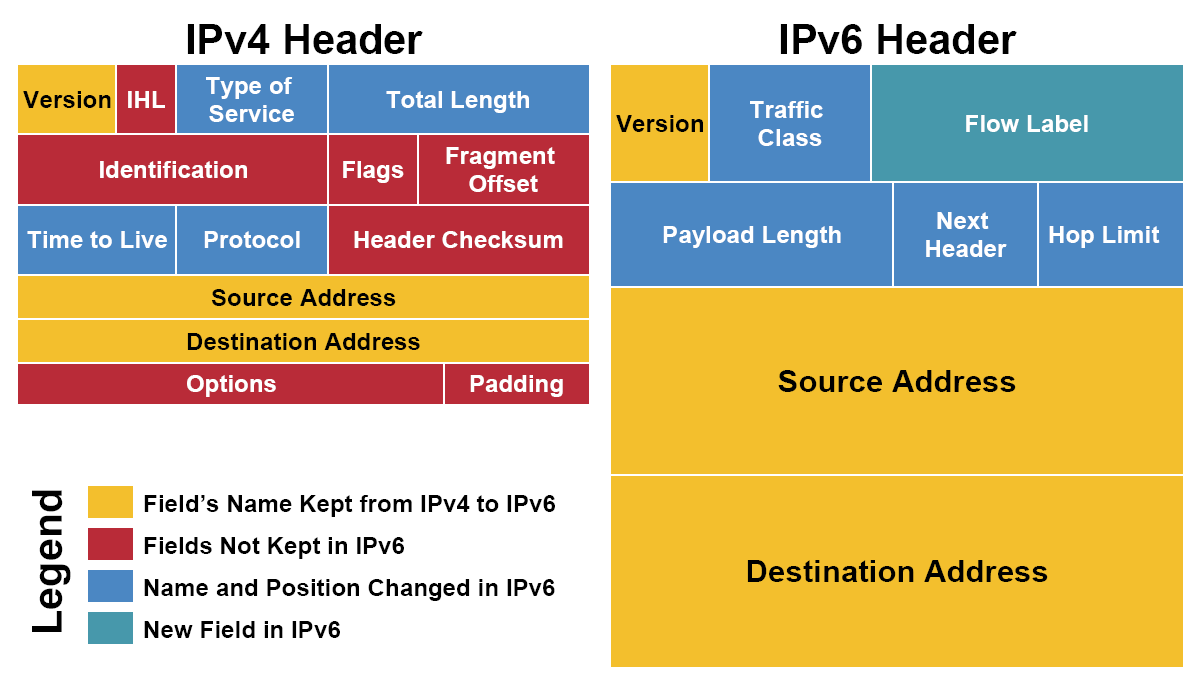
\includegraphics[height=4.5cm]{Semernik2}
  \caption{Формат заголовков пакетов IPv4 и IPv6. ~\cite{Semernik-3}}
\end{figure}


Формат IPv6 адреса отличается от формата IPv4 адреса и состоит из следующих основных частей (на примере адреса 2001:db8:f3d:1::1):

\begin{table}[h!]
  \centering
  \begin{tabular}{ l l l }
    2001:0db8:0f3d  & :0001  & :0000:0000:0000:0001  \\
     Site prefix (48 bit)  &  Subnet ID (16 bit)  &  Interface ID (64 bit)  \\
  \end{tabular}
\end{table}
Site prefix обычно назначается провайдером или регистратурой и спользуется при маршрутизации. Subnet ID используется в топологии сети клиента, а Interface ID назначается на клиентские устройства автоматически либо вручную.

Различают полную и сжатую (compressed) формы записи IPv6 адресов. При этом существует два основхных правила сжатия формы записи:

\begin{enumerate}
  \item Лидирующие нули (слева) в пределах квартета (4 байта) могут не указываться.
  \item Любое количество идущих подряд нулей можно заменить на ::, но только один раз. Если в адресе присутсвуют две одинаковые по длине последовательности нулей разделенных любым другим числом, на :: заменяется та, что находится левее.
\end{enumerate}

Примеры:
2001:0db8:0ffc:0008:0000:0000:0000:002f ~--- полная форма записи
2001:db8:ffc:8::2f ~--- сжатая форма записи
2001:0db8:0000:0000:0001:0000:0000:0001 ~--- полная форма записи
2001:db8::1:0:0:1 ~--- сжатая форма записи

При доступе к IPv6 адресу через URL необходимо использовать квадратные кавычки. Пример: \url{ http://[2001:db8:ffff::2]:8081}.

В IPv6 появились такие новые понятия как области адресов (address scopes) и специальные адреса. Сегодня активно используется более 16 специальных адресов (например, loopback, unspecified, uniq local addresses, есть даже отдельные адреса для целей документации ~--- 2001:db8::/32) и 7 основных областей адресов (global scope, link-local scope, interface-local и др.)

Адрес IPv6 может быть вручную сконфигурирован на сетевом интерфейсе, либо назначен автоматически с помощью механизма SLAAC, заложенного в сам протокол. Так же поддерживается автоматическое назначение IPv6 адресов с помощью DHCPv6-сервера. Для выдачи клиенту не одного адреса, а определённой сети (префикса) широко используется DHCPv6 Prfix Delegation. ~\cite{Semernik-4} Любой сетевой интерфейс в современных операционных системах всегда имеет сконфигурированный автоматически IPv6 адрес с областью действия link-local.

В отличает от протокола IPv4, работа которого базируется на протоколе ARP, в IPv6 ипользуется ICMP unicast и milticast.

Координационный центр европейского сообщества пользователей сети Интернет ~--- RIPE NCC подготовил серию OnLine-курсов, которые являются хорошим началом на пути освоения нового протокола IPv6. ~\cite{Semernik-5}
\begin{thebibliography}{20}
\bibitem{Semernik-0}\url{https://ru.wikipedia.org/wiki/IPv6}
\bibitem{Semernik-1}\url{https://www.youtube.com/watch?v=s61g\_l9NoR8, Alex Semenyaka, RIPE NCC}
\bibitem{Semernik-2}\url{https://www.google.com/intl/en/ipv6/statistics.html}
\bibitem{Semernik-3}\url{https://343networks.files.wordpress.com/2010/06/ipv4-ipv6-header.gif}
\bibitem{Semernik-4}\url{https://en.wikipedia.org/wiki/Prefix\_delegation}
\bibitem{Semernik-5}\url{https://academy.ripe.net/course/view.php?id=2} , требуется регистрация на сайте сообщества.
\end{thebibliography}
\end{document}
